\documentclass[language=en,sheet=4,prefix]{exercise}

\exerciseCourse{Development of Safety Critical Systems(Sichere Software)}
\exerciseAuthors{Martin Leucker, Grigory Markin, Felix Lange}
\exerciseTerm{winter term 18}
\exerciseDeadline{}


\usepackage{utf8-math}
\usepackage{xspace}
\usepackage{tikz}
\usetikzlibrary{arrows,automata}


\newcommand{\ltl}{LTL}
\renewcommand{\phi}{\varphi}

% Temporal operators
\newcommand{\U}{\ensuremath{\operatorname{U}}\xspace}
\newcommand{\XU}{\ensuremath{\operatorname{XU}}\xspace}
%\newcommand{\R}{\ensuremath{\operatorname{R}}\xspace}
\newcommand{\X}{\ensuremath{\operatorname{X}}\xspace}
\newcommand{\WX}{\ensuremath{\operatorname{\bar{X}}}\xspace}
\newcommand{\G}{\ensuremath{\operatorname{G}}\xspace}
\newcommand{\F}{\ensuremath{\operatorname{F}}\xspace}
\newcommand{\W}{\ensuremath{\operatorname{W}}\xspace}


\begin{document}

\task[Linear-time temporal logic]

Specify the following properties of linear executions using \ltl
\begin{itemize}
    \item ``$p$ holds in the third position.''
    \item ``$p$ never holds.''    
    \item ``$p$ holds before the third position or it never holds.''
    \item ``$p$ holds from the beginning until $q$ holds.''    
    \item ``$p$ holds from the beginning until $q$ holds and $q$ has to hold sometime.''
    \item ``$p$ holds at most, as long as $q$ holds.''
    \item $\{w ∈ Σ^ω\ |\ ∀_{i∈ℕ}  \{p,q\}\subseteq w_i \}$
    \item $\{w ∈ Σ^ω\ |\ ∃_{i∈ℕ}  \{p,q\}\subseteq w_i \}$
    \item $Σ^ω$
    \item $∅$
\end{itemize}

%----------------------------------------------------------------------------------

\begin{solution}
\begin{itemize}
  \item $\X\X p$
  \item $\G\neg p$
  \item $p \vee \X p \vee \G\neg p$
  \item $p \W q$
  \item $p \U q$
  \item $p \U \neg q$
  \item $\G (p \wedge q)$
  \item $\F (p \wedge q)$
  \item $true$
  \item $false$
\end{itemize} 
\end{solution}

%----------------------------------------------------------------------------------
%----------------------------------------------------------------------------------
%----------------------------------------------------------------------------------

\task[Labeled Transition System]
Consider the following labeled transition system.

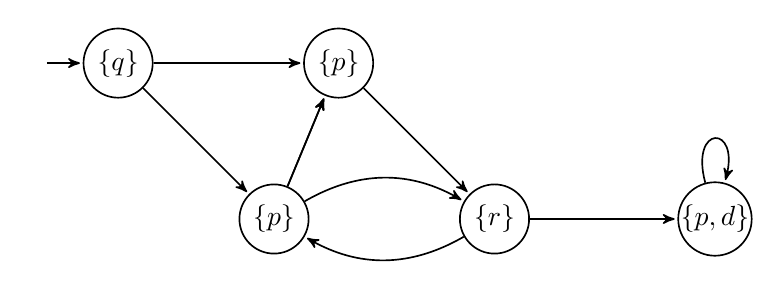
\begin{tikzpicture}[->,>=stealth',shorten >=1pt,auto,node distance=2.8cm,
                    semithick, initial text=]
  \tikzstyle{every state}=[draw=black,text=black, inner sep = 0]

  \node[initial,state] (A)                    {$\{q\}$};
  \node[state]         (B) [right of=A] {$\{p\}$};
  \node[state]         (D) [below right of=A] {$\{p\}$};
  \node[state]         (C) [below right of=B] {$\{r\}$};
  \node[state]         (E) [right of =C]       {$\{p,d\}$};

  \path (A) edge (B);
  \path (A) edge (D); 
  \path (B) edge (C);
  \path (D) edge (B);
  \path (C) edge (E);
  \path (C) edge [bend left] (D);
  \path (D) edge (B);
  \path (D) edge [bend left] (C);
  \path (E) edge [loop above]  (E);
\end{tikzpicture}

  
Which of the following properties hold in \emph{all} executions of the transition system ?

\begin{minipage}[t]{\textwidth}
  \begin{minipage}{.4\textwidth}
    \begin{itemize}
      \item $p$
      \item $\F d$
      \item $¬\F d$
      \item $\G\F p$
      \end{itemize}
  \end{minipage}
  \begin{minipage}{.4\textwidth}
    \begin{itemize}
      \item $\F\G(p\U q)$
      \item $q \U ¬(p\U d)$
      \item $\G(p \rightarrow \X\F p)$
      \item $\X\X\X p$
      \end{itemize}
  \end{minipage}
\end{minipage}
%----------------------------------------------------------------------------------
\begin{solution}
\begin{minipage}[t]{\textwidth}
  \begin{minipage}{.4\textwidth}
    \begin{itemize}
      \item No
      \item No (There exists a cycle without d)
      \item No ($¬\F d \equiv \G \neg d$)
      \item Yes (in the loop at the last state $p$ always hold)
      \end{itemize}
  \end{minipage}
  \begin{minipage}{.4\textwidth}
    \begin{itemize}
      \item No (after $p$ is reached, there is no way to go back to $q$)
      \item Yes (all paths after $q$ towards $d$ go through $r$)
      \item Yes (if $p$ does not hold, that's fine, but after $p$ holds, there is always some position where $p$ holds again)
      \item No (e.g. $q p r$)
      \end{itemize}
  \end{minipage}
\end{minipage}
\end{solution}


%----------------------------------------------------------------------------------
%----------------------------------------------------------------------------------
%----------------------------------------------------------------------------------

\task[Symbolic Encoding]

Consider the labeled transition system from the previous Task.
\begin{itemize}  
\item How many variables do we need to encode the transition system in propositional logic ?
\item Define the set of propositional variables $V$ and describe the set of initial states and the transition relation by propositional formulas $I$ and $T$ respectively.
\item Consider LTL properties from the previous task that do not hold for the considered transition system. Find for every the properties the lowest bound $k$ (if there exists one) that is enough to falsify the property using the Bounded Model Checking algorithm.  
\end{itemize}

%----------------------------------------------------------------------------------
%----------------------------------------------------------------------------------
%----------------------------------------------------------------------------------

\begin{solution}
\begin{itemize}
  \item We have 5 states, i.e. we need at least $3$ propositional variables. It's enough to encode $2^3$ states. 
  \item For the sake of clarity, we encode every state by a separate variable (from left to right, starting from the first row): $S = \{ s_0, s_1, s_2, s_3, s_4\}$. Variables for atomic propositions: 
  $AP = \{ p, q, r, d \}$. Finally, the set of variables is defined as $V = S \cup AP$.
  \item Initial states: $I(V) = s_0 \wedge q \wedge \bigwedge_{v \in V \setminus \{ s_0, q \}} \neg v$  
  \item Let: 
    \begin{itemize}
      \item $T_{s_0 \rightarrow s_1}(V, V') = s_0 \wedge s_1' \wedge p'  \wedge \bigwedge_{v \in V' \setminus \{ s_1', p' \}} \neg v'$            
      \item $T_{s_0 \rightarrow s_2}(V, V') = s_0 \wedge s_2' \wedge p'  \wedge \bigwedge_{v \in V' \setminus \{ s_2', p' \}} \neg v'$
      \item $T_{s_1 \rightarrow s_3}(V, V') = s_1 \wedge s_3' \wedge r'  \wedge \bigwedge_{v \in V' \setminus \{ s_3', r' \}} \neg v'$      
      \item $T_{s_2 \rightarrow s_1}(V, V') = s_2 \wedge s_1' \wedge p'  \wedge \bigwedge_{v \in V' \setminus \{ s_1', p' \}} \neg v'$
      \item $T_{s_2 \rightarrow s_3}(V, V') = s_2 \wedge s_3' \wedge r'  \wedge \bigwedge_{v \in V' \setminus \{ s_3', r' \}} \neg v'$
      \item $T_{s_3 \rightarrow s_2}(V, V') = s_3 \wedge s_2' \wedge p'  \wedge \bigwedge_{v \in V' \setminus \{ s_2', p' \}} \neg v'$
      \item $T_{s_3 \rightarrow s_4}(V, V') = s_3 \wedge s_4' \wedge p' \wedge d'  \wedge \bigwedge_{v \in V' \setminus \{ s_4', p', d' \}} \neg v'$
      \item $T_{s_4 \rightarrow s_4}(V, V') = s_4 \wedge s_4' \wedge p' \wedge d'  \wedge \bigwedge_{v \in V' \setminus \{ s_4', p', d' \}} \neg v'$
    \end{itemize}
    \item Then transition relation is defined as:
      \begin{align*}
      T(V, V') = & 
        T_{s_0 \rightarrow s_1}(V, V') \vee T_{s_0 \rightarrow s_2}(V, V') \vee \\
        & T_{s_1 \rightarrow s_3}(V, V') \vee T_{s_2 \rightarrow s_1}(V, V') \vee \\
        & T_{s_2 \rightarrow s_3}(V, V') \vee T_{s_3 \rightarrow s_2}(V, V') \vee \\
        & T_{s_3 \rightarrow s_4}(V, V') \vee T_{s_4 \rightarrow s_4}(V, V') \\
      \end{align*}
    \item Following properties from the previous task does not hold:
      \begin{itemize}
        \item $p$
        \item $\F d$       
        \item $¬\F d$
        \item $\F\G(p\U q)$
        \item $\X\X\X p$
      \end{itemize}
    \item Bounds to falsify properties using BMC (NOTE: we need to negate every property and show that negated property holds within first $k$ steps):
      \begin{itemize}
        \item $k = 0$ ($\neg p$ is true in the initial state) 
        \item $k = INF$ ($\neg \F d \equiv \G \neg d$ cannot be fulfilled, because we never know if in the next states $d$ could hold (without loop recognition))
        \item $k = 3$ ($\neg \neg \F d \equiv \F d$ is true after $\{q\},\{p\},\{r\},\{p,d\}$)
        \item $k = INF$ ($\neg\F\G(p \U q) \equiv \G\F \neg (p \U q)$) we need loop recognition to show that $p \U q$ never holds)
        \item $k = 3$ ($\X\X\X p$ is true after $\{q\},\{p\},\{p\},\{r\}$).
      \end{itemize}      
\end{itemize}
\end{solution}

\end{document}
